\documentclass{standalone}
\usepackage{tikz}
\usetikzlibrary{positioning, quotes}
\begin{document}
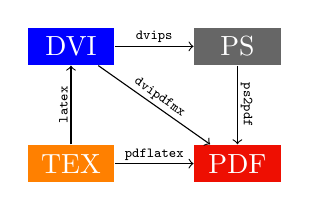
\begin{tikzpicture}[
    every node/.style = {text=white, minimum width=1.1cm},
    every edge/.style = {draw, ->},
    every edge quotes/.style = {text=black, auto=left, font=\ttfamily\tiny, sloped, inner sep=1pt}
]
    \node (tex) [fill=orange] {TEX};
    \node (pdf) [fill={rgb:red,244;green,15;blue,2}, right=of tex] {PDF};
    \node (dvi) [fill=blue, above=of tex] {DVI};
    \node (ps) [fill=black!60, above=of pdf] {PS};

    % \draw (tex) edge["pdflatex"] (pdf)
    %     (tex) edge["latex"] (dvi)
    %     (dvi) edge["dvips"] (ps)
    %     (dvi) edge["dvipdfmx"] (pdf)
    %     (ps) edge["ps2pdf"] (pdf);

    \draw (tex) edge["pdflatex"] (pdf)
            edge["latex"] (dvi)
        (dvi) edge["dvips"] (ps)
            edge["dvipdfmx"] (pdf)
        (ps) edge["ps2pdf"] (pdf);
\end{tikzpicture}
\end{document}